\renewcommand{\baselinestretch}{1.5}
\fontsize{12pt}{13pt}\selectfont

\chapter{SLAM系统设计} \label{System Overview}
本章节主要介绍SLAM的概念和原理、一个基本SLAM系统的框架、两个优秀的开源SLAM框架和地图融合算法。

\section{SLAM系统}
同时定位与建图(SLAM,simultaneous localization and mapping)技术,其希望是机器人在对环境和自身所处在环境中的位置未知的情况下,在反复的运动过程中不断观测到的地图特征完成自身位置的定位和姿态的确定,之后再根据自身位置对环境构建增量式的地图,从而达到同时定位与建图的目的。


\subsection{成像原理及相机参数} \label{3.1.2}
在各种SLAM中,视觉SLAM由于其传感器(光学相机)造价较低的原因,成为了SLAM中最常用的方式,要了解使用相机的视觉SLAM的原理,首先需要了解相机的成像原理及其参数。

如图\ref{fig4},可以用小孔成像的原理简单地解释针孔相机的模型:
\begin{figure}[!ht]
	\centering
	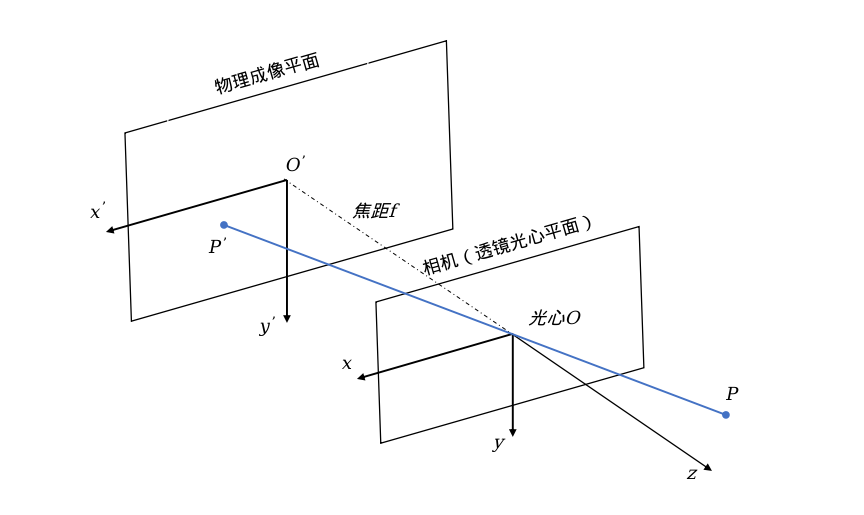
\includegraphics[width=0.6\textwidth]{camera.png}
	\caption{针孔相机模型} 
	\label{fig4}
\end{figure}

$Oxy$平面为相机光心(垂直主光轴)所在的平面,称其为相机平面,对应的$O-x-y-z$坐标系即为相机坐标系;$O'x'y'$平面为物理成像平面,$\bar{OO'}$的长度为焦距$f$;在现实世界中有一点$P$,设其在相机坐标系下的坐标为$[X, Y, Z]^T$,其经过小孔$O$投影后,在相机坐标系下落在像素平面上的坐标为$[X', Y', Z']^T$。

理论下,小孔成像为倒立的实像,但在实际的相机中,成像被人为旋转,成正立的像,因此不考虑坐标系正负号的影响,由相似三角形关系,有:

\begin{equation}
\frac{Z}{f}=\frac{X}{X'}=\frac{Y}{Y'}
\end{equation}


在此基础上,定义像素坐标系。像素坐标系为二维坐标系,在物理成像平面上;像素坐标系的原点位于图像的左上角,横轴为$u$轴,向右与$x$轴平行,纵轴为$v$轴,向下与$y$轴平行,则可以得到像素坐标与$P'$坐标的关系为:

\begin{equation}
\begin{cases}
u=\alpha X'+c_x=\alpha f \cfrac{X}{Z}+c_x \\
v=\beta Y' +c_y=\beta f  \cfrac{Y}{Z}+c_y \\
\end{cases}
\end{equation}


其中,$\alpha$和$\beta$为横轴和纵轴的缩放倍数,$c_x$为图像横向像素的一半,$c_y$为图像纵向像素的一半。令$f_x=\alpha f$,$f_y=\beta f$,将像素坐标系下的坐标转换为齐次坐标:

\begin{equation}
\begin{bmatrix}
u\\v\\1
\end{bmatrix}=
\frac{1}{Z}
\begin{bmatrix}
f_x & 0 & c_x\\
0   & f_y & c_y\\
0 & 0 & 1
\end{bmatrix}
\begin{bmatrix}
X\\Y\\Z
\end{bmatrix}=
\frac{1}{Z} \bf{KP}
\end{equation}


则得到了相机的内参矩阵(Camera Intrinsics)$\bf{K}$。通常情况下,对于焦距固定的相机(或定焦镜头),其出厂之后内参矩阵是固定的;如果无法从厂家得到相机的内参,可以使用标定的方法获得相机的内参矩阵,常见的标定算法有张正友标定法\cite{Gao2017SLAM}。

除相机的内参外,还有相机外参(Camera Extrinsics)的定义;相机的外参由其旋转矩阵$\bf{R}$和平移向量$\bf{t}$构成。对于$P$点而言,其在相机坐标系(像素坐标平面)下的坐标应为其在世界坐标系下的坐标根据相机相对于世界坐标系的位姿所变换得到的,相机的位姿即由其外参决定,则世界坐标系下$P$点的坐标$\bf{P_w}$在相机坐标系下的坐标为:


\begin{equation}
Z
\begin{bmatrix}
u\\v\\1
\end{bmatrix}=
\bf{K(RP_w+t)}
\end{equation}

\subsection{视觉SLAM的基本步骤} \label{3.1.3}

经典的视觉SLAM框架如图\ref{fig5}所示:

\begin{figure}[!ht]
	\centering
	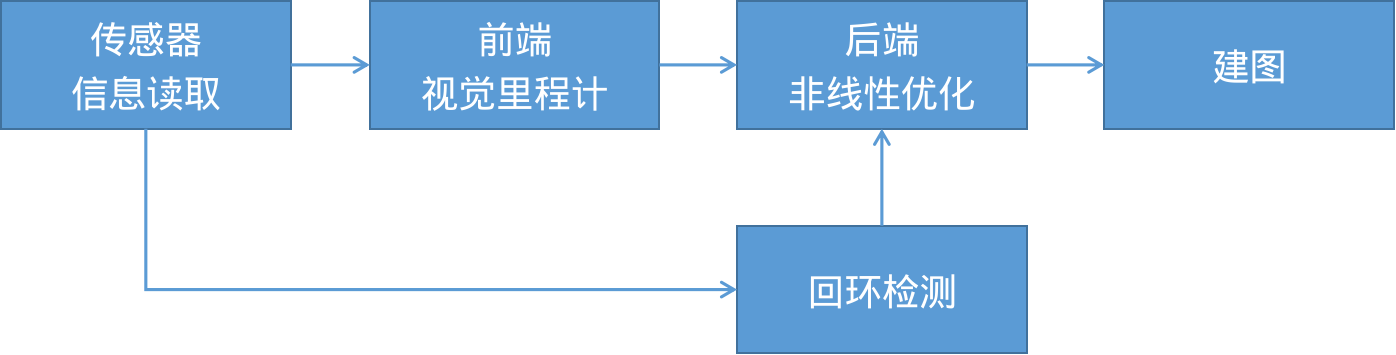
\includegraphics[width=0.7\textwidth]{SLAM.png}
	\caption{经典视觉SLAM框架} 
	\label{fig5}
\end{figure}

经典视觉SLAM流程包括以下基本步骤:
\begin{enumerate}
	\item 
	传感器信息读取。主要为相机图像的读取以及一些预处理步骤,在不同的视觉SLAM算法中,可能还涉及惯性测量元件信息的读取和预处理。
	\item 
	前端视觉里程计(Visual Odometry)。视觉里程计的功能是从相邻的几帧图像之中,根据几何约束,得到相机的运动;并且通过记录地图点(路标)与相机的相对位置,构建局部地图。
	\item 
	后端(非线性)优化(Optimization)。后端主要涉及滤波与非线性优化算法,其目的是减少传感器的误差,完成对运动的相机和周围环境的不确定性的估计。
	\item 
	回环检测(Loop Closure Detection)。回环检测的作用是使机器人能够分辨出当前面临的场景是否曾经来到过,解决位置估计的误差随时间累计,发生漂移的问题;并且消除累计误差,最终得到全局一致的轨迹和地图。
	\item 
	建图(Mapping)。建图即根据前端里程计和后端优化得到的地图点(路标点),构建地图。
\end{enumerate}

% 视觉里程计
视觉里程计是SLAM的关键,其基本完成了同时定位与建图的任务。视觉里程计的实现主要有两种方法:特征点法和直接法。

% 特征点法
特征点法作为很长时间以来视觉里程计的主要方法,其特点是比较稳定,在光照差异大和画面中有动态物体的情况下也能较好地完成任务。特征点法的核心在特征点的提取与匹配;提取即从每帧图像中找到可以代表图像特征的点,辨识度更高的点。

\begin{figure}[!ht]
	\centering
	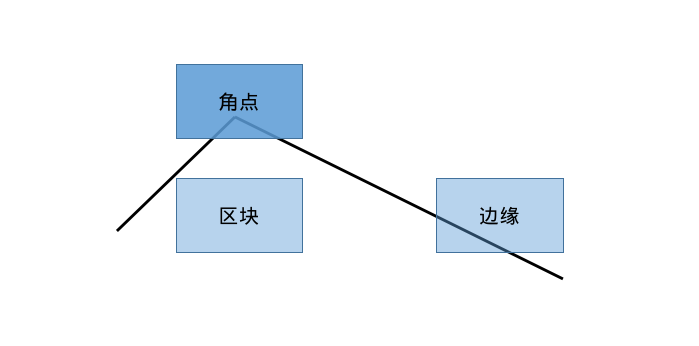
\includegraphics[width=0.6\textwidth]{corner.png}
	\caption{角点、边缘、区块} 
	\label{fig6}
\end{figure}

特征点的一种方法是使用角点。如图\ref{fig6},可以把一张图像中的内容分为角点、边缘、区块三种类型。可以发现,指出某两张图像中出现的统一区块是最难以实现的,因为存在大面积相同的色块,无法确定具体点的匹配;其次是边缘,其具有一定的特征,但沿边缘行进,仍可能出现相同的局部特征,造成误匹配;因此选择其中最具有特征角点作为特征。性能较好、比较稳定的角点有SIFT、SURF,ORB等。

% 对极几何与三角测量
在完成特征点提取与匹配后,根据不同的传感器类型,有不同的得到相机位姿的方法。对于传统的单目相机传感器,可以使用对极几何约束,得到相机的运动,并通过三角测量的方法恢复地图点相对于每时刻相机的位置。

% 直接法
前端视觉里程计的另一种方法是直接法,由光流法演变而来。光流法与特征点法不同,特征点法使用特征点的描述子来完成特征匹配,而光流法可以跟踪特征点的运动,这样就无需进行大量的描述子匹配运算。直接法可以弥补特征点法的一些缺陷。


% 优化
后端优化主要有两种方法,滤波和非线性优化。拓展卡尔曼滤波EKF及其演变出的粒子滤波方法等,在早期的SLAM设计中应用十分广泛。但随着非线性优化方法的普及,现在的SLAM方案多用BA图优化及位姿图优化的方法,并且有可以使用的ceres和g2o库。

% 回环检测
回环检测在判断场景是否曾经来过时,一般用的是词袋模型(Bag of Words)\cite{zhang2010understanding},根据图像中是否存在同样的几种相似特征来判断是否在外观上相似。

% 建图
建图根据地图的需求,可以分为用于定位的稀疏地图,用于导航、重建的稠密地图和用于交互的语义地图。按照地图的分类,可以分为拓扑地图和度量地图两种;拓扑地图着重与图节点之间的连通性,而度量地图则能够精确地表示出地图点相对于相机的位置。


%\subsection{对极几何约束与三角测量} \label{3.1.4}


\section{ORB-SLAM2}

ORB-SLAM2是由萨拉戈萨大学的Raúl Mur-Artal开发,可以用在单目、双目、RGB-D深度相机的视觉SLAM系统。

\subsection{ORB特征点及描述子} \label{3.2.1}

% 简单介绍 
ORB特征点是上文\ref{3.1.3}提到过的特征点的一种,它的全称是Oriented FAST and Rotated BRIEF;其中,FAST是角点的一种,BRIEF是Binary Robust Independent Elementary Feature,是一种二进制描述子;ORB特征点即由改进的FAST关键点和带旋转的BRIEF描述子组成。

% FAST
FAST角点选取的核心思想是,选取的点和周边像素点亮度差别很大,则该点可能是FAST角点。如图\ref{fig7}所示,对于可能被选取为FAST角点的像素点$p$,其亮度为$I_p$;设置亮度差异的阈值$T$,可以为$0.3I_p$;选取半径为3的圆上的16个点,对应图中的16个深色点,记录各点的像素值$I_i$,如果16个点中有连续$N$个点满足$|I_i-I_p|>T$,则像素点$p$可以被认为是FAST角点,该标准为FAST-N,N一般取9、11、12\cite{Gao2017SLAM}。

\begin{figure}[!ht]
	\centering
	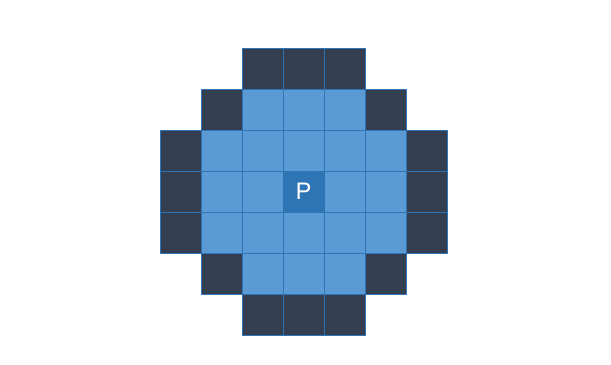
\includegraphics[width=0.5\textwidth]{FAST.png}
	\caption{FAST角点} 
	\label{fig7}
\end{figure}

% Oriented FAST
单纯的FAST关键点是不带方向性的,为了准确性,ORB的Oriented FAST关键点给FAST角点添加了方向和尺度的描述。其尺度的描述是由计算机视觉中构建金字塔模型的方法,在不同分辨率的图像下都能够提取到特征点,而旋转的描述则是由灰度质心法实现的,如图\ref{fig8}所示:

\begin{figure}[!ht]
	\centering
	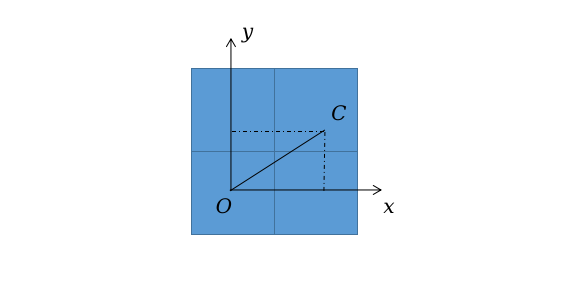
\includegraphics[width=0.5\textwidth]{OFAST.png}
	\caption{灰度质心法}
	\label{fig8}
\end{figure}

设$O$为角点像素,取一个最小的图像块,只有四个像素构成,建立$O-x-y$坐标系,原点的像素用$I(0,0)$表示,则可以找到该图像块的质心为:

\begin{equation}
C=(\frac{I(1,0)}{I(0,0)}, \frac{I(0,1)}{I(0,0)})
\end{equation}

则可以得到方向向量$\vec{OC}$,该关键点的方向定义为:

\begin{equation}
\theta = \arctan{\frac{I(0,1)}{I(1,0)}}
\end{equation}


% BRIEF
BRIEF描述子为二进制编码,反映了关键点附近128个像素对的大小关系,最终由0和1构成,其具有旋转不变性、选点速度快且易于存储。


\subsection{ORB-SLAM2的配置}
% config
ORB-SLAM2是标准的CMake工程,这就意味着其可以使用CMake进行配置并且进行make编译;其虽然支持ROS,但并不是ROS的catkin工程,使用的是rosbuild相关命令,而不是ROS常见的catkin make编译指令。

ORB-SLAM2的github主页上,详细介绍了其编译的方法,官方将编译代码集成到了build.sh文件中;正常情况下,可以通过chmod +x命令给该sh文件赋予可执行权限后,运行sh命令,直接编译。如图\ref{fig10}所示,需要编译的内容为两个第三方库和ORB-SLAM2主要函数;需要注意的是,make -j命令指的是只用全部线程进行编译,这样做可能会造成电脑资源锁死,可以根据电脑的配置自行修改所用线程数。

\begin{figure}[!ht]
	\centering
	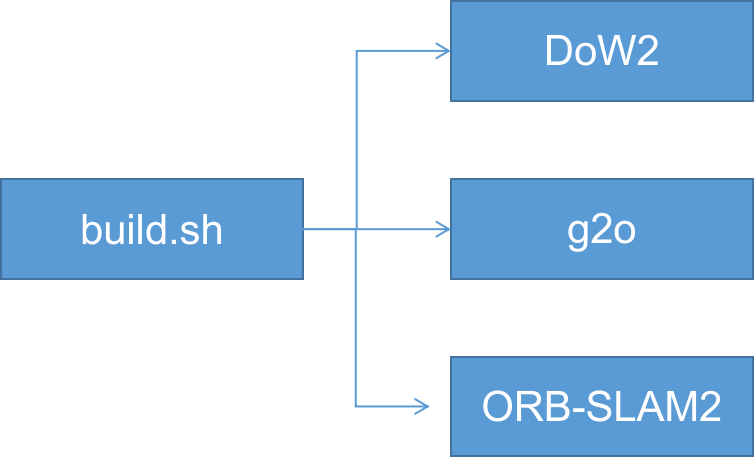
\includegraphics[width=0.45\textwidth]{build.png}
	\caption{配置ORB-SLAM2}
	\label{fig10}
\end{figure}

ORB-SLAM2在普通编译过程中,可能会遇到一些问题:
\begin{enumerate}
	\item System.cc中,usleep未定义;这是由于System.h文件中缺少头文件unistd.h导致的,加上该头文件即可。
	\item 
	找不到Eigen3库;大概率是因为Pangolin版本为0.6,但ORB-SLAM2使用的Pangolin版本为0.5;一种方法是将Pangolin版本退回0.5,另一种方法是将CMakeList.txt中的Eigen3 REQUIRED改为REQUIRED NO\_MODULE。如果仍然找不到Eigen3库,如果是用Eigen3源代码编译安装的非模板类Eigen3库,则可以通过ln -s建立软链接的方式,在ORB需要找到Eigen3的位置添加上Eigen3的库。
	\item 
	Eigen3的问题,在ROS编译的CMakeList中也需要修改。
\end{enumerate}

普通编译完成后,使用TUM数据集进行测试,从System.cc中可以得出,在终端中需要三个参数:ORB字典的路径、相机配置文件的路径、数据集的路径。

由于需要在ROS环境下使用,首先执行build\_ros.sh。之后需要添加环境变量给ROS工作空间,即在.bashrc文件中,添加上ROS功能包的路径,指向Examples/ROS文件夹。至此,ORB-SLAM2在普通环境和ROS环境下均配置完成。

\subsection{ORB-SLAM2整体框架}

ORB-SLAM2在运行时,其整体框架如图\ref{fig-ORBstructure}所示,可以看出,系统主要由3个并行的线程构成,分别为跟踪、本地建图和回环。
~\\
\begin{figure}[!ht]
	\centering
	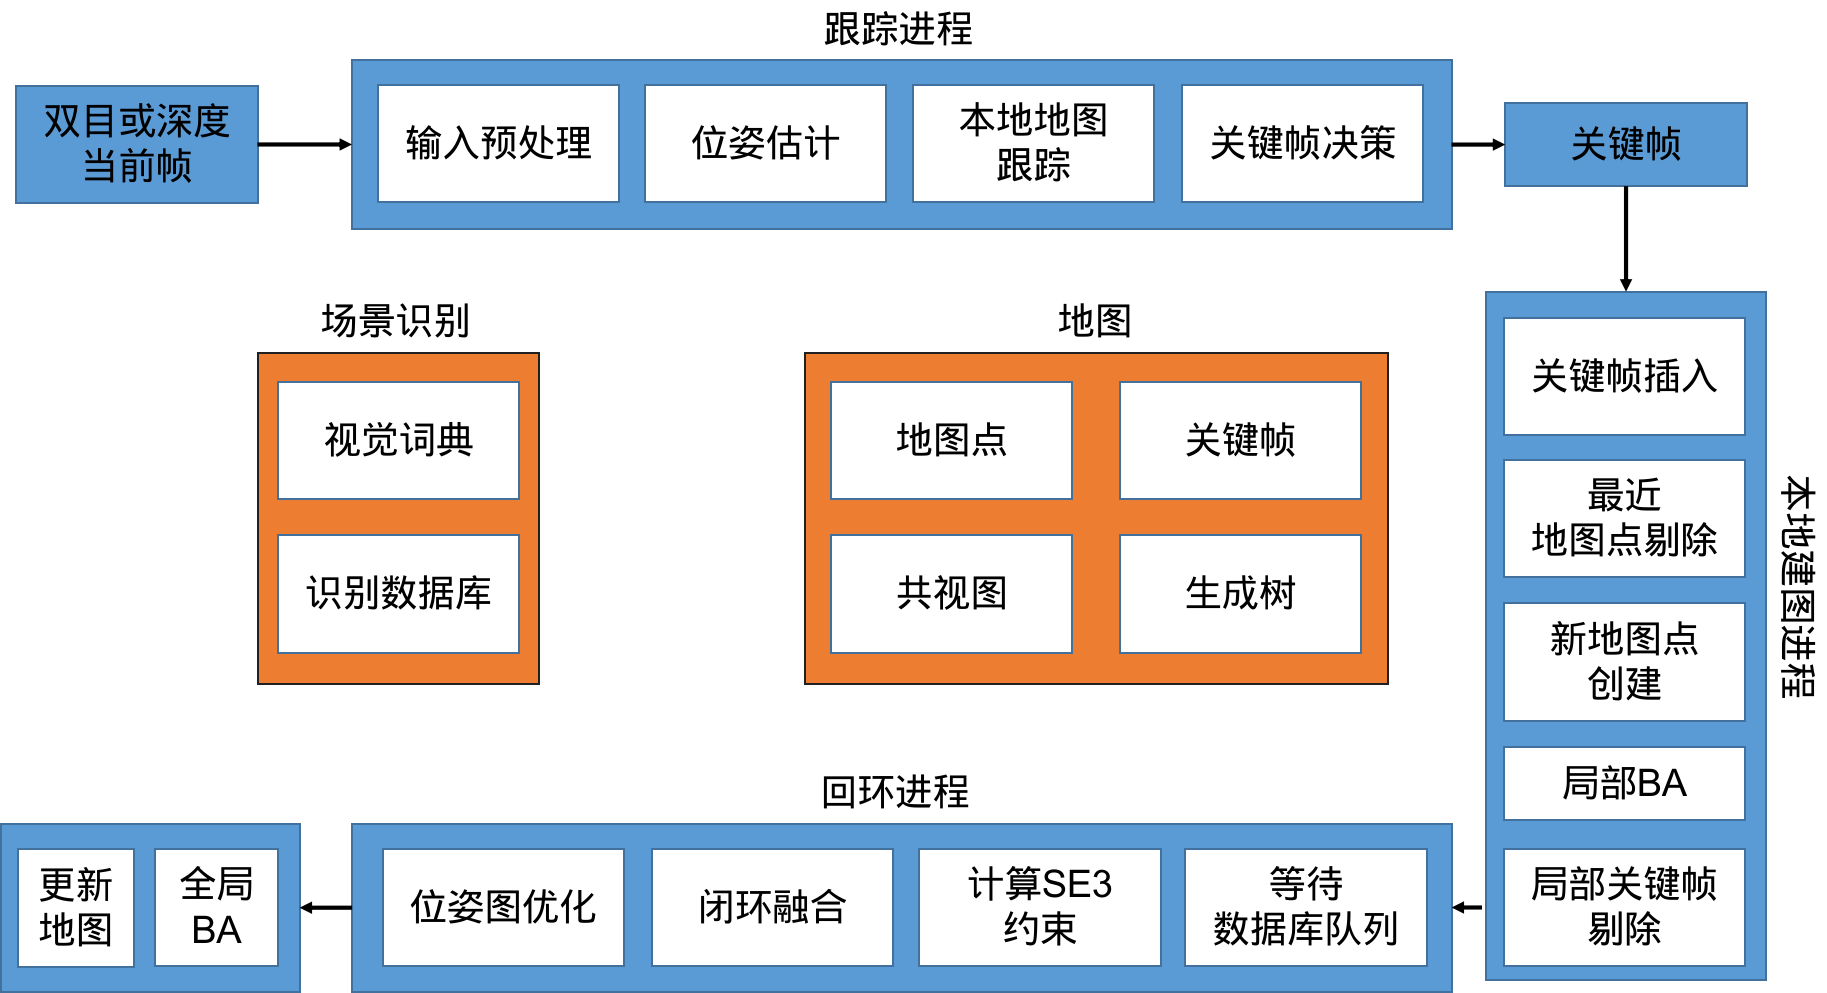
\includegraphics[width=0.94\textwidth]{ORBstructure.png}
	\caption{ORB-SLAM2整体框架}
	\label{fig-ORBstructure}
\end{figure}

跟踪线程的目的是从相机观察到的每一帧获取相机当前的位置;在过程中根据与本地地图的特征点匹配,仅使用运动估计的BA来最小化重投影误差。首先进入到当前帧的预处理阶段,在这一部分中,将会完成对当前帧的ORB特征点提取与匹配环节,最终得到满足要求的关键点;之后是根据运动跟踪模型或重定位的方法建立对当前相机位姿的估计,并与本地地图建立联系,得到在地图中的跟踪,并最终决定该帧是否可以作为关键帧插入到关键帧数据库中。

本地建图线程的目的是管理本地地图并且进行局部BA,做出优化。在整个ORB-SLAM的运行中,共有三种BA。一是在跟踪线程中的基于运动模型的BA,二是在本地地图中优化关键帧和地图点的局部BA,和最后回环检测完成后的全局BA,这些都是用的是基于g2o的LM信任域收敛优化方法。在该线程中,输入的内容为关键帧,首先要完成关键帧的插入,其次是剔除一些最近的不符合要求的地图点,而后建立一些新的地图点,并且开始局部BA优化,最后会选择剔除一些关键帧。

回环线程的目的是完成回环检测、通过位姿图优化消除累计误差;检测到闭环并完成合并后,会开启全局BA线程,优化全局的路径。在经历本地建图线程后,关键帧会进入回环线程;首先是回环检测,在这之中需要进行SE3的计算,要求不仅满足相似关系,还要满足几何约束的关键帧才能进入到回环的闭环修正中;当进入到修正阶段,融合闭环后,则要进行位姿图优化。在这之后,开启新的全局优化进程,进行全局BA优化,并且更新优化后的地图。

除此之外,系统还嵌入了基于BoW2的场景识别模块,并将其用于重定位。对于回环检测,系统保留了共视图模型,其串联了两个具有共视关系的关键帧;另外设有一个连接各个关键帧的最小生成树。这些设计使得ORB-SLAM2能够在大场景中正常工作,并且当闭环结束后为位姿图优化提供框架。



\subsection{ORB-SLAM2的主要模块} \label{3.2.2}

ORB-SLAM2是一套规范完整的视觉SLAM系统,其主要模块可以分为四个:跟踪模块、本地地图模块、回环检测进程、可视化模块\cite{mur2017orb}。如图\ref{fig9}所示,从以下五个主要函数中分析。

\begin{figure}[!ht]
	\centering
	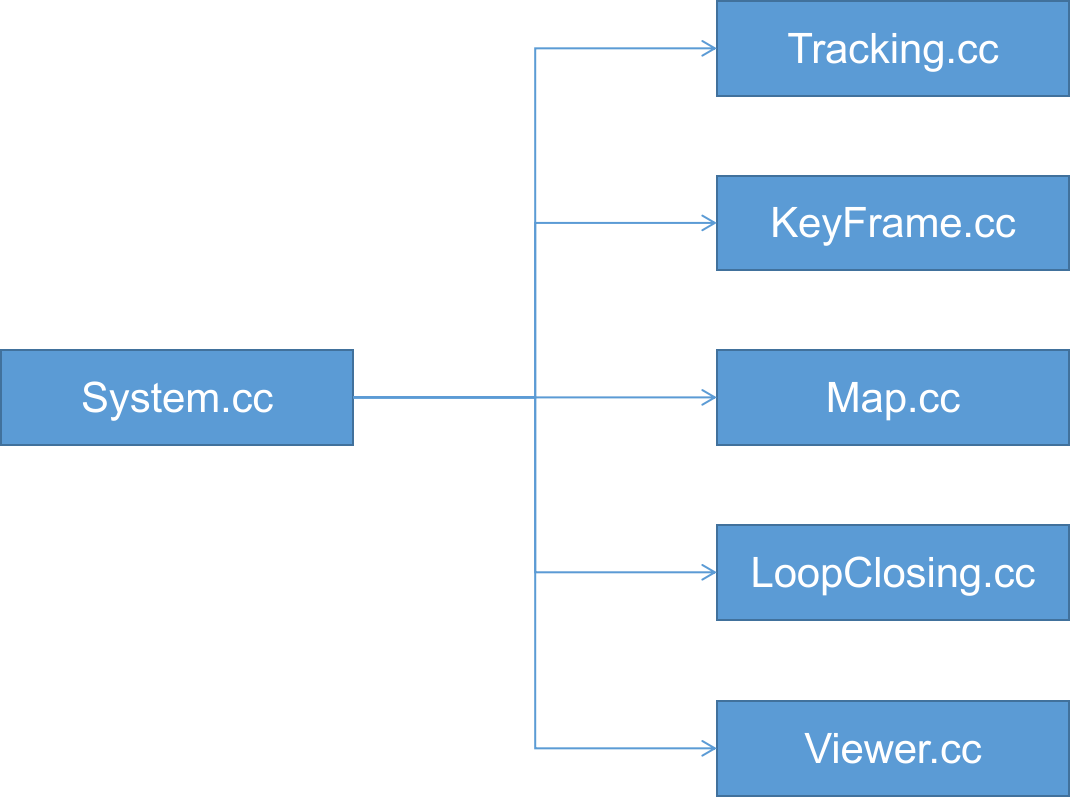
\includegraphics[width=0.65\textwidth]{ORB2.png}
	\caption{ORB-SLAM2主要模块}
	\label{fig9}
\end{figure}

% System
\textbf{System.cc},SLAM系统顶端控制:

首先是读取ORB词典,该词典是配合DoW2库训练得到的,用于回环检测时判断图像的外观相似度。

其次是创建ORB特有的KeyFrameDatabase,该类用于处理关键帧数据;创建地图,实例化Map对象;创建画笔,为可视化做准备。

\begin{minted}[fontsize=\small]{cpp}
//Create KeyFrame Database
mpKeyFrameDatabase = new KeyFrameDatabase(*mpVocabulary);

//Create the Map
mpMap = new Map();

//Create Drawers. These are used by the Viewer
mpFrameDrawer = new FrameDrawer(mpMap);
mpMapDrawer = new MapDrawer(mpMap, strSettingsFile);
\end{minted}

之后是主要线程的初始化,跟踪线程、本地地图线程和回环检测线程:
\begin{minted}[fontsize=\small]{cpp}
//Initialize the Tracking thread
//(it will live in the main thread of execution, the one that called this constructor)
mpTracker = new Tracking(this, mpVocabulary, mpFrameDrawer, mpMapDrawer,
mpMap, mpKeyFrameDatabase, strSettingsFile, mSensor);

//Initialize the Local Mapping thread and launch
mpLocalMapper = new LocalMapping(mpMap, mSensor==MONOCULAR);
mptLocalMapping = new thread(&ORB_SLAM2::LocalMapping::Run,mpLocalMapper);

//Initialize the Loop Closing thread and launch
mpLoopCloser = new LoopClosing(mpMap, mpKeyFrameDatabase, mpVocabulary, mSensor!=MONOCULAR);
mptLoopClosing = new thread(&ORB_SLAM2::LoopClosing::Run, mpLoopCloser);
\end{minted}

System相当于工程中的Main函数,汇集了实现一个SLAM系统所需的全部流程,使用顶层的代码进行控制,具体功能则由底层的类及其中的函数去实现。

% Tracking
\textbf{Tracking.cc},关键的跟踪进程,其主要函数为图像的转换函数和Track主函数:
\begin{enumerate}
	\item 
	图像转换函数是针对不同传感器设置的,以单目相机为例;该函数需要判断图像是否为灰度图,判断图像为RGB或BGR编码,并最后将图像转为系统使用的灰度3通道图像,赋予其时间戳和ORB字典、相机的内参矩阵和畸变参数等信息,构成当前帧的对象。
	\item 
	Track函数,该函数是Tracking.cc中的主要函数,或称之为顶端函数。该函数首先判断系统状态,之后根据状态选择使用运动模型或里程计模型得到当前位姿,以及是否需要重定位;如果得到相机位姿和正确匹配,则依次在建立的Map中跟踪路标、将路标更新到画笔中、判断是否将该帧加入关键帧、清除里程计的匹配和未跟踪的MP。
\end{enumerate}

% KeyFrame
\textbf{KeyFrame.cc},该类的操作都基于关键帧进行:

\begin{enumerate}
	\item 
	共视图;确定关键帧之间的共视关系,该内容将被用于优化及回环检测,最终建立一个关键帧之间的共视图关系。
	\item 
	地图点;还包括MP地图点的添加与移除、跟踪与匹配等;
	\item 
	位姿;包括获取位姿、旋转矩阵$\bf{R}$,平移向量$\bf{t}$等;
\end{enumerate}

% Loop Closing
\textbf{LoopClosing.cc},回环检测的主要函数:

\begin{enumerate}
	\item 检测是否有新的关键帧;在此之前要给回环的队列加互斥锁,之后返回逻辑变量,表示是否有新的关键帧;
	\item 检测是否有闭环;提取出一个关键帧,并用互斥锁加锁,防止被擦除;之后对地图进行判断,如果地图包含少于10个关键帧,则直接判定为没有闭环;使用具有共视关系的关键帧基于词袋模型进行评分,将共视关键帧得到的最高分作为最低分;最后删除其他的闭环候选帧,暂时找到与当前关键帧一致的关键帧。
	\item 计算相似变换;Sim3算法,其结果是得到两帧之间的相对位姿,只有Sim3求解器得到足够多的匹配点,才能接受该闭环帧。
	\item 融合位姿图。
\end{enumerate}



\section{CCM-SLAM}

% introduction of CCM
CCM-SLAM是由苏黎世联邦理工大学Patrik Schmuck开发,其含义是中心式协同单目视觉SLAM。
其特点是适用于多个设备(最多四个)同时运行,并且有一个终端负责管理控制和处理数据,是一种联合协同式的SLAM方案。

\subsection{CCM-SLAM的结构} \label{3.3.1}

CCM在算法上使用了ORB-SLAM2的方法,保留了其跟踪、关键帧、关键帧数据库、Sim3求解等类;与此同时,更加明确了自己的Client+Server机制,其核心是中心式的协同结构和各设备之间的通信方法。

\begin{figure}[!ht]
	\centering
	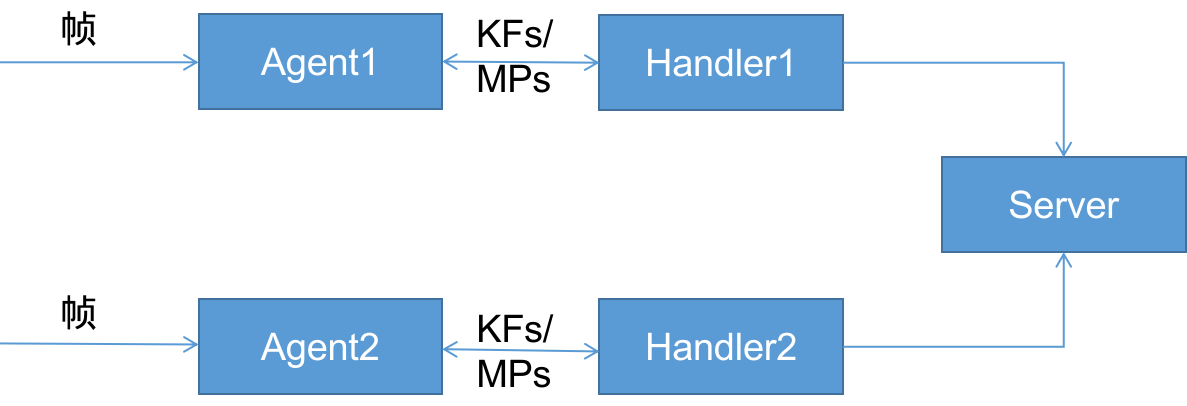
\includegraphics[width=0.8\textwidth]{CCMstructure.png}
	\caption{CCM-SLAM框架}
	\label{fig11}
\end{figure}

% detailed CCM info
如图\ref{fig11}所示,CCM的核心是其将整个系统的SLAM进程分为了Client和Server两个模块处理。应用了网络中的客户端与服务器模型,这里的客户端指的是携带相机传感器的各设备终端,设备的种类可以是无人机、无人车、无人船甚至改进的手持相机,而服务器一般是一台中央处理电脑。

设备作为客户端,其并不是一个简单的相机加图片数据传输,而是一个有一定复杂的的运算系统。在客户端中,需要接收传感器得到的帧信息,并且做里程计运算,得到关键帧,通过通信模块将数据发送给服务器中负责接收信息的处理单元;除此之外,在客户端中还存储有建立的局部地图,地图点保持与服务器的地图数据库更新。

关键帧和地图点的数据进入服务器的信息处理单元后,地图点直接进入服务器的地图存储库中;对于新的关键帧,如果能够检测到地图场景重叠,则直接进入到优化过程,并将优化后的结果存储到地图存储库中;该关键帧正常情况下会进入地图匹配和地图融合模块,之后再进入优化环节,随后存储到库中;如果所有客户端都到达相同的场景,则最后地图存储库只会有一张地图\cite{schmuck2019ccm}。

\subsection{Client与Server机制} \label{3.3.2}

CCM-SLAM主要有两大板块的内容,一部分是地图的处理,另一部分是其客户端和服务器的机制及通讯方式。

客户端的设计可以分为三步,如图\ref{fig12}所示,整体的流程是由ClientNode到ClientSystem再到ClientHandler,其中的引用关系即为该流程。

\begin{figure}[!ht]
	\centering
	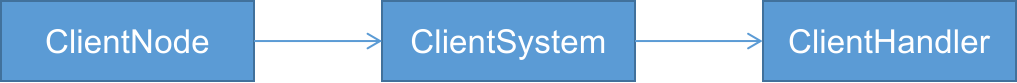
\includegraphics[width=0.6\textwidth]{Client.png}
	\caption{Client设计}
	\label{fig12}
\end{figure}

ClientNode负责的内容包括:ROS节点初始化,句柄的设计,使用指针创建ClientSystem。在ROS节点的初始化过程中,使用的节点名称是CSLAM client node;值得注意的是其句柄的设计,一般的ROS句柄都实例化NodeHandler,但其又实例化了NodeHandler("~"),该操作旨在给相机和地图等话题之前加上节点的名称,以于不同的终端作区分;最后使用了智能指针,创建了ClientSystem对象,意味着对该客户端创建了属于其自己的客户端系统。

\begin{minted}[fontsize=\small]{cpp}
ros::init(argc, argv, "CSLAM client node");

if(argc != 3){
    cerr << "Usage: rosrun cslam clientnode path_to_vocabulary path_to_cam_params";
    ros::shutdown();
    return 1;
}

ros::NodeHandle Nh;  // topic name will be: node name(only), like "/image_raw"
// topic node will be: node name + topic name, like "iris_0/image_raw"
ros::NodeHandle NhPrivate("~"); 

boost::shared_ptr<cslam::ClientSystem> pCSys{new
                cslam::ClientSystem(Nh,NhPrivate,argv[1],argv[2])};
\end{minted}

ClientSystem负责的内容包括:读取ID,SLAM初始化及预先数据准备。首先从ROS的参数服务器读取客户端ID,使用ROS的param方法读取该数据;之后进行标准的SLAM数据预先准备流程,即加载词典、创建关键帧数据库、创建地图;最后进行初始化步骤,在这里引入了ClientHandler。

\begin{minted}[fontsize=\small]{cpp}
int ClientId;
// get ClientID from launch file, actually ROS parameter server
mNhPrivate.param("ClientId",ClientId,-1);
mClientId = static_cast<size_t>(ClientId);
// assign ClientID to member of class ClientSystem, mClientID

// load vocabulary
this->LoadVocabulary(strVocFile);

// Create KeyFrame Database
mpKFDB.reset(new KeyFrameDatabase(mpVoc));

// Create the Map
mpMap.reset(new Map(mNh,mNhPrivate,mClientId,eSystemState::CLIENT));
usleep(10000); //wait to avoid race conditions

// Initialize Agent
mpAgent.reset(new ClientHandler(mNh,mNhPrivate,mpVoc,mpKFDB,mpMap,
mClientId,mpUID,eSystemState::CLIENT,strCamFile,nullptr));
usleep(10000); //wait to avoid race conditions
mpAgent->InitializeThreads();
usleep(10000); //wait to avoid race conditions
\end{minted}

ClientHandler负责的内容包括:向总地图中添加该ID客户端的地图,定义Sim3转换,将该ID客户端的相机话题名加载到ROS的参数服务器,最后开始了具体的初始化。


%\subsection{CCM-SLAM的配置}

%与ORB-SLAM2相同,CCM-SLAM在其github上有详细的编译方法;与ORB-SLAM2不同的是,CCM-SLAM是完全的catkin架构,完全基于ROS,所以其必须被放置在ROS工作空间的src文件夹下,并且使用catkin make命令编译CCM-SLAM工程。需要注意的是最好不要使用全部线程进行编译。


\section{地图融合方案}

地图的融合原理与回环检测类似,但不同于回环检测,地图融合在识别出场景重叠后,不止需要完成定位,还要对重叠场景的地图点完成归类和补充。

\subsection{系统框架} \label{3.4.0/}

\begin{figure}[!ht]
	\centering
	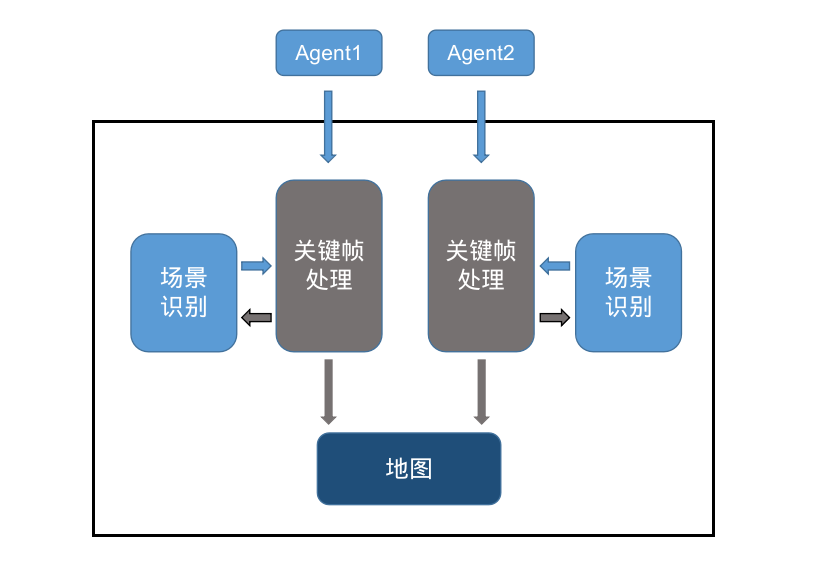
\includegraphics[width=0.7\textwidth]{csfm.png}
	\caption{系统框架}
	\label{fig13}
\end{figure}

地图融合系统的框架如图\ref{fig13}所示:无人机1和无人机2将帧信息传递给系统的关键帧处理单元,关键帧处理单元对帧做出处理,首先筛选出其中的关键帧,没有入选的帧则被舍弃。

筛选出的关键帧随后首先进入到场景识别模块,该处的作用类似回环检测,即识别出相似的场景,这一点仍然使用基于外观的相似检测,即使用BoW的词袋模型。如果没有探测到场景重叠(注意,相邻的关键帧不会被并入考虑是否重叠,除了很大概率存在重叠外,在代码的逻辑中还需剔除共视关键帧的影响),则进入正常的优化和回环检测、建图等环节;如果探测到场景重叠,则需要视情况而定\cite{forster2013collaborative}:

\begin{figure}[!ht]
	\centering
	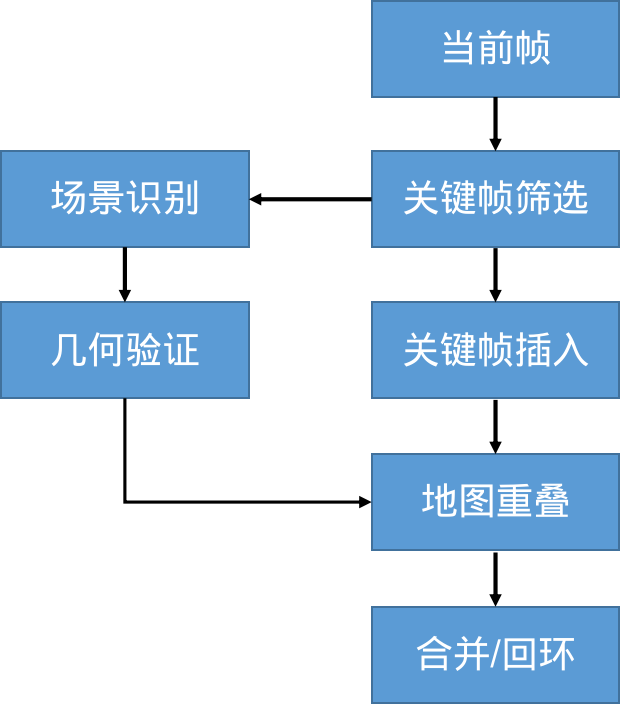
\includegraphics[width=0.35\textwidth]{keyframe.png}
	\caption{关键帧处理}
	\label{fig-keyframe}
\end{figure}

\begin{enumerate}
	\item 若该场景与本机已经经历过的场景重合,则不进入地图拼合模块,直接进入优化和回环检测模块;对重叠的定义需要判断是完全重叠或部分重叠,若完全重叠则也会进入到回环检测模块;若连续几帧均为部分重叠,即说明对某些点保持跟踪,而在SLAM进程中只有连续几帧都可见的路标点才会被计入地图点,属于正常跟踪进程。
	\item 若该场景与本机的场景无重合,在与另一架无人机的场景识别中探测到重叠,则会进入到地图融合进程;
\end{enumerate}


\subsection{场景识别} \label{3.4.1}

当关键帧被确定后,其首先要进行场景识别检测;检测的对象来自关键帧数据集,其在SLAM进程中不断扩充,因此需要使用一种运算速度快的场景识别方法。本研究中使用基于外观相似判断的BoW2算法。

BoW即Bag of Words,意为单词的集合。算法的核心原理是将图像中出现的各元素进行划分,出现的元素算作一个单词,则整张图片变成了单词的合集;众多图片中单词的合集构成了字典。
随后根据不同类型的元素组成一个向量,因此复杂的图像描述就被转换成了简单的向量描述。

假设当前拥有一个包含三个单词的字典,三个单词为$\omega_1, \omega_2, \omega_3$,并且有图片$I$,图片中仅有元素$\omega_2$,则该图片可以表示为下式:

\begin{equation}
I = 0 \cdot \omega_1 + 1 \cdot \omega_2 + 0 \cdot \omega_3
\end{equation}

转换为向量描述,则有$I=[0, 1, 0]^T$;由此,只要拥有一个足够全面的字典,就可以使用这种方法描述一张图片;如果不考虑图片中元素出现的次数,而只关注出现与否,则该向量简化为了一个二维向量。当面对两张图像的相似度比较时,可是根据两张图像向量差来判定相似度,还有很多计算相似度的方法。

BoW字典的生成使用了无监督聚类的K-means方法,通过大量图片计算各种特征的特征点,将具有某一类特征的特征点构成一个组合,也就构成了一个单词;只要在查找时对应到该单词为最相似的单词,则可以认为找到了一个元素。但是字典由大量单词构成,如果直接查找则不能满足SLAM实时性的要求,因此需要使用特殊的数据结构,比如k叉树。

\begin{figure}[!ht]
	\centering
	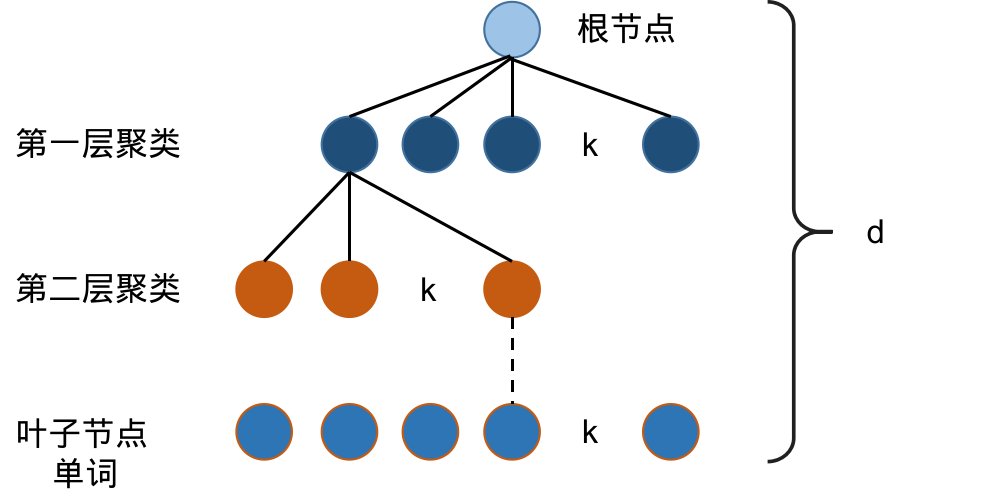
\includegraphics[width=0.8\textwidth]{ktrees.png}
	\caption{k叉树字典}
	\label{fig-ktrees}
\end{figure}

图\ref{fig-ktrees}表示了一个k叉树字典的构成;图中的圆表示不同的特征,圆之间的连线代表在查找某种特征时的路径。最上方的是根节点,首先使用k-means聚类方法把N个特征点分为k类,由此构成了第一层聚类;之后同理,根据不同特征聚类,最终构成了d层,每个节点在下一层又拥有k类的树状结构,这样的k叉树可以存储$N=k^d$个单词,并且使用分级的方式查找也能够保证效率和实时性。

接下来需要的是对相似度给出量化的方法。使用TF-IDF思想,其含义为在图像中经常出现的和在字典中较少出现的单词,都具有很高的区分度。在进行相似度计算时,区分度高的单词,其权重也高,这样带有权值地计算会有更好的效果。

首先,在建立字典时可以统计某叶子节点$\omega_i$的IDF值,假设共有$n$个特征,该叶子节点出现的次数为$n_i$,则有其IDF值为:

\begin{equation}
IDF_i=\log{\frac{n}{n_i}}
\end{equation}

可以看出,$n_i$的值越小,则其IDF评分越高。

其次计算其TF值,假设在某图像中,该叶子节点的特征出现了$n_i$次,该图像拥有的总单词数为$n$,则有其TF值为:

\begin{equation}
TF_i=\frac{n_i}{n}
\end{equation}

可以看出,$n_i$的值越大,则其TF评分越高。

可以定义叶子节点特征$\omega_i$的权重$W_i$为:

\begin{equation}
W_i = TF_i \times IDF_i
\end{equation}

对于某一叶子节点特征,如果能在图像中获得其权重,以此类推,则可以获得图像中所有单词的权重,根据此可以得到带有权重的BoW向量,以图片I为例,则其BoW向量$v_I$为:

\begin{equation}
v_I = [(\omega_1, W_1), (\omega_2, W_2), ... , (\omega_N, W_N)]
\end{equation}

完成场景识别后,如果属于自身的地图,则最终会参与到本机的全局BA优化中;如果属于其他终端的地图,则会进入地图融合模块。


\subsection{地图融合} \label{3.4.2}

地图融合的前提是存在场景相似,并且当前帧与数据库中的关键帧可以获得一定的匹配关系。如图\ref{fig-mapmerge}所示:现有匹配的关键帧1与关键帧2及其各自的地图1与地图2,地图合并首先会创建一个新地图,在此称其为“总地图”,由地图1和地图2中的点构成。

\begin{figure}[!ht]
	\centering
	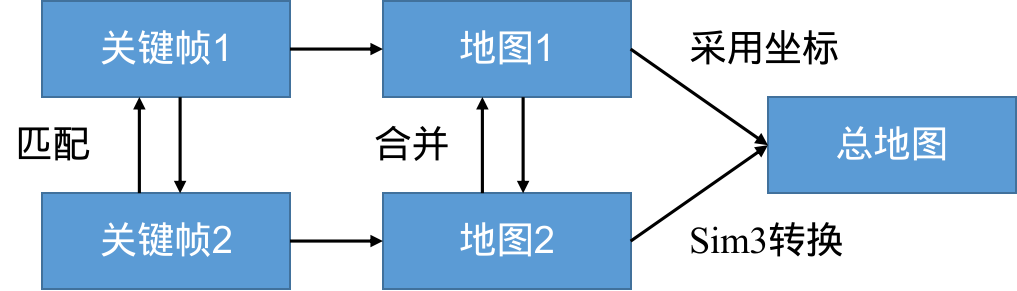
\includegraphics[width=0.6\textwidth]{mapmerge.png}
	\caption{融合方法框架}
	\label{fig-mapmerge}
\end{figure}

假设地图1的坐标系被“总地图”所采用,则地图1的所有地图点直接进入到总地图中,但是地图2中的点需要完成12之间的坐标系相对转换关系,才能将2中的地图点也复制到“总地图”中。在地图1与地图2中,匹配的地图点会直接合并成一个地图点,放到“总地图”中,而未匹配的地图点则会根据Sim3转换复制到“总地图”坐标系中,并且会产生新的约束关系。

具体的几何视角,如图\ref{fig14}所示,将两张图像中的地图点进行特征点匹配操作;对于图中的地图点,其在两个坐标系下,通过三角测量得到的坐标是不一致的,由此推得两个坐标系的转换关系,从而以一个无人机坐标系为主,将另一个坐标系中的点进行坐标变换后,重复的点舍弃,新增的点则按照坐标系转换关系补充到地图中,从而完成地图融合。

\begin{figure}[!ht]
	\centering
	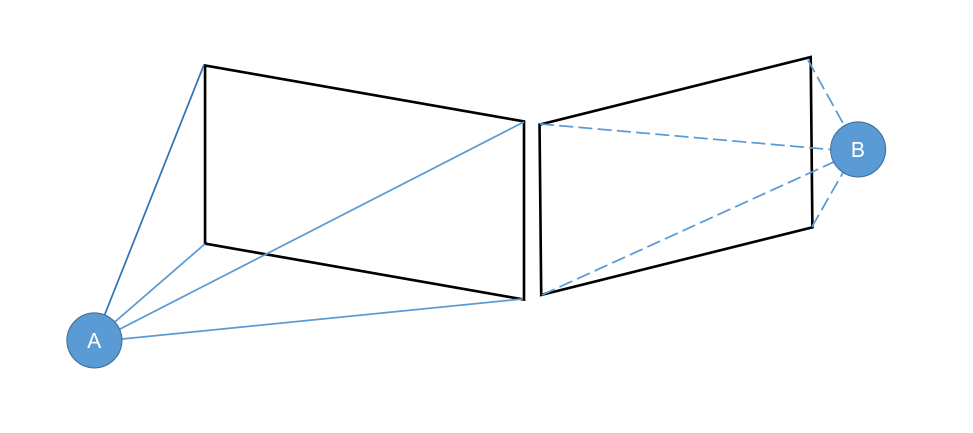
\includegraphics[width=0.6\textwidth]{theory.png}
	\caption{地图点匹配}
	\label{fig14}
\end{figure}

设有四张包含场景重叠但在不同位置拍摄的图片,随机对其分为2组,一组的图片序号为1,2;二组图片的序号为3,4;

对两组图片首先进行ORB特征点提取,之后使用提取和匹配到的特征点,计算两组相机运动的位姿变换矩阵,为$T_{12},T_{34}$,则现有两套坐标转换关系,并且可以根据三角测量的方法,获得两组地图点相对于各自参考图片(1,3)的位置$P_{12},P_{34}$;

由于该场景包含重叠场景,我们默认其符合拼接地图的要求;接下来对1,3进行特征点提取和匹配,并随后计算1,3之间的转换矩阵$T_{13}$,则可以由此矩阵,将1中的地图点转换到3坐标系下:

\begin{equation}
P_{12-3}={\bf R_{13}} \times P_{12} + \bf{t_{13}}
\end{equation}

这一部分的代码实现如下,其中,shiftCoordinate函数为实现上式的函数。

\begin{minted}[fontsize=\small]{cpp}
// get KeyPoint position of Client0 in Client1
vector<Point3d> map_point0_1;
map_point0_1 = ORBMatcher::shiftCoordinate(R, t, K, map_points0);
map_point0_1.insert(map_point0_1.end(), map_points1.begin(), map_points1.end());
// show combination map
ORBMatcher::showMapPoints(map_point0_1);

vector<cv::Point3d> ORBMatcher::shiftCoordinate(const Mat &R, const Mat &t, const Mat &K,
const vector<cv::Point3d> &pos) {
    // Pos_new = (RP + t)
    vector<Point3d> shiftedPos;
    Point3d p;

    Eigen::Matrix<double, 3, 3> Mat_R;
    Eigen::Matrix<double, 3, 1> Mat_t;
    Eigen::Matrix<double, 3, 1> Mat_P;
    Eigen::Matrix<double, 3, 3> Mat_K;
    Eigen::Matrix<double, 3, 1> Mat_Pos;

    cv2eigen(R, Mat_R);
    cv2eigen(t, Mat_t);

    for (const auto & po : pos){
        Mat_Pos << po.x, po.y, po.z;
        Mat_P = Mat_R * Mat_Pos + Mat_t;
        p.x = Mat_P(0);
        p.y = Mat_P(1);
        p.z = Mat_P(2);
        shiftedPos.push_back(p);
    }
    return shiftedPos;
}
\end{minted}

实现点云绘制的为showMapPoints函数,主要使用了Pangolin库,使用OpenGL对各点进行绘制并且给出可交互窗口。其中的关键循环如下:

\begin{minted}[fontsize=\small]{cpp}
for (const auto & MapPoint : MapPoints){
    glVertex3d(MapPoint.x, MapPoint.y, MapPoint.z);
}
\end{minted}

由此获得了简单的拼合场景;

\begin{figure}[htbp]
	\centering
	\begin{minipage}[t]{0.45\columnwidth} %小于1/n如果使用n张图片
		\centering
		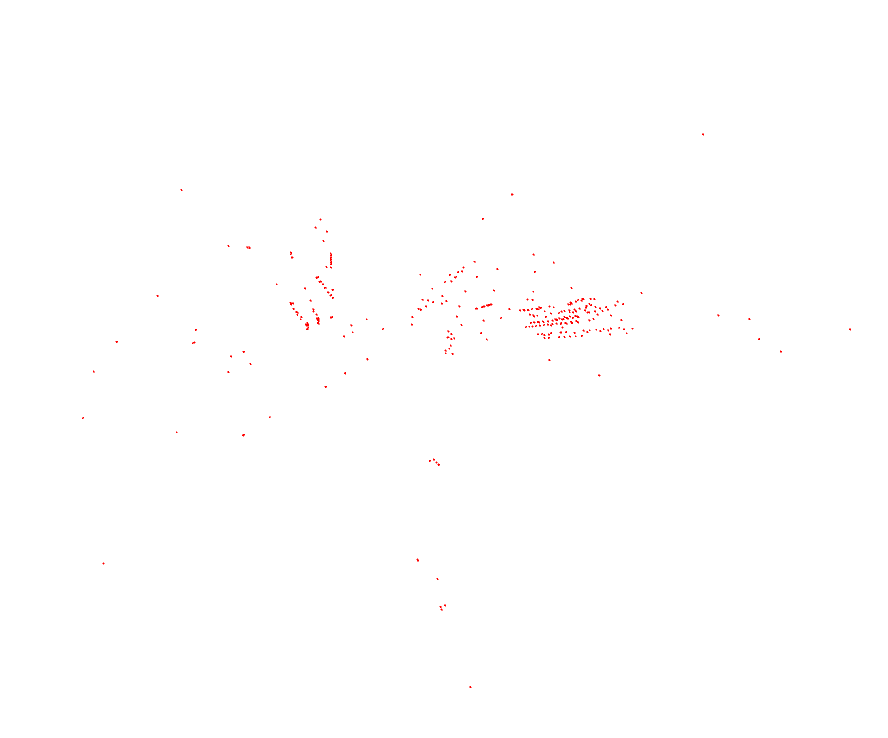
\includegraphics[width=0.8\columnwidth]{merge3.png}
		\caption{单独地图点}
		\label{merge1}
	\end{minipage}
	\begin{minipage}[t]{0.45\columnwidth}
		\centering
		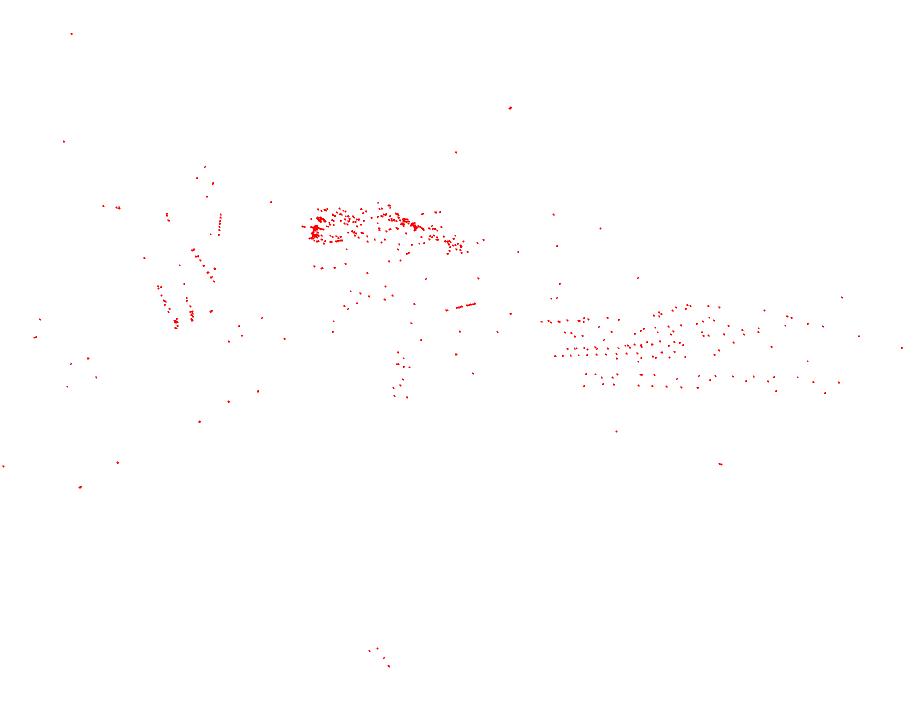
\includegraphics[width=0.8\columnwidth]{merge4.png}
		\caption{合并地图点}
		\label{merge2}
	\end{minipage}
\end{figure}









